\documentclass[conference]{IEEEtran}

\usepackage{cite}
\usepackage{amsmath,amssymb,amsfonts}
\usepackage{algorithmic}
\usepackage{graphicx}
\usepackage{textcomp}
\usepackage{xcolor}
\usepackage{pdfpages}

\graphicspath{ {./pics/} }

\def\BibTeX{{\rm B\kern-.05em{\sc i\kern-.025em b}\kern-.08em
    T\kern-.1667em\lower.7ex\hbox{E}\kern-.125emX}}
\begin{document}

\title{meet\&do: Meeting website for students and enthusiasts\\}

\author{\IEEEauthorblockN{Stanislas Lange}
\IEEEauthorblockA{\textit{Dept. of Computer Science} \\
\textit{Hanyang University}\\
Seoul, South Korea\\
stanislas@hanyang.ac.kr}
\and
\IEEEauthorblockN{Simon Gaussmann}
\IEEEauthorblockA{\textit{Dept. of Industrial Engineering} \\
\textit{Hanyang University}\\
Seoul, South Korea\\
simongaussmann6658@web.de}
\and
\IEEEauthorblockN{Stéphane Rabenarisoa}
\IEEEauthorblockA{\textit{Dept. of Computer Science} \\
\textit{Hanyang University}\\
Seoul, South Korea\\
rabena.stephane@gmail.com}
\and
\IEEEauthorblockN{Marc-Antoine Dariel}
\IEEEauthorblockA{\textit{Dept. of Information Systems} \\
\textit{Hanyang University}\\
Seoul, South Korea\\
marc-antoine.dariel@cpe.fr}
}

\maketitle

\begin{abstract}
meet\&do is a website that aims to put people in touch who have similar interests and hobbies or need help with issues related to their studies. 
Enthusiasts can find each other through the website and share real-life activities together.
\end{abstract}

\section{Introduction}

Nowadays, we are more connected than ever through social media and all kinds of internet-based services yet somehow people are still isolated from each other. 
Forming friendships and relationships has become challenging for some as it is easy and convenient to hide behind a social media profile. 
Everyone has an online presence. 
In this environment, many may find themselves isolated and looking for real-life interactions.

We want to create a website that aims at putting people in touch who have similar interests and hobbies or need help with issues related to their studies. 
Getting in touch online is easy but that is just the first step. 
After finding people with the same interests and making appointments, users of our website meet in real life. 
Meeting new people works best if you are already interested in similar fields and activities and we want to put people together who have those in common. 
Common interests to bond over and meet up again in the future or form new friendships.

Where already existing alternatives might take a more generic approach, we want to create a solution that gives users the opportunity to choose what they are looking for from the beginning. 
Therefore, the website will be divided into four main areas. 
That makes it less confusing and easy and intuitive to navigate.

\section{Alternatives}


\subsection{Jodel}

Jodel is a Social Media platform from Germany that aims particularly at university students and connecting people who are in the same area. 
User’s can share content, however events as such can’t be created. 
It is only available on mobile operating systems and has no website. 
Users in an area can’t see posts other than those made locally. 
Posts are assigned colors which are chosen randomly. 
The platform is available in several languages and European countries.

\subsection{Meetup.com}

 Meetup is the competitor with the most similarities to our project. 
 The website offers a service used to organize online groups that host real life events for people with similar interests. 
 Events of all kinds can be hosted which don’t have to conform to certain categories. 
 Also, event organizers have to pay a fee to host events. 
 The website is available in many languages.

\subsection{Others}

Various other social networks like Facebook that also include the feature to create and host events. 
In essence, all social media platforms fulfill similar functions that aim at communication and gathering people. 
Some of them, like Facebook, have inbuilt Event Managers to create and host events. 
Others, like Instagram and Twitter, allow users to track events and participating people via hashtags.

Differentiating aspects of MeetnDo: While Jodel restricts the user’s view to their local area and is not suitable to host events, our project aims at events that can be hosted anywhere the user chooses and offering a clear and user friendly interface which is color coded by event type for a more organized experience. 
Also, Meetup.com takes a wider and more generic approach which is something we want to avoid in order to make the service more accessible and less overwhelming. 
For that reason our service offers preset categories that make it easy for the user to determine whether they are potentially interested in an event.

\section{Technical specification}

\subsection{Software used}

The website will be built using Ruby 2.6 and the framework Ruby on Rails 6.0. We chose Ruby and Rails because we like the simplicity of the language and we want to expand our knowledge on this framework. 
Ruby on Rails allows us to save time for CRUD (Create, read, update and delete) operations and allows us to focus on feature that differentiate our website. 
Moreover, Ruby on Rails follows the MVC architecture (Model, View, Controller) which will help us keep our code clean and organized in a specific folder arborescence and separate our code depending on its use (models, controllers, routes, helpers, and so on.

Rails also enables us to implement a REST API which can be used if we use a front end Javascript framework like Vue.js or if we end up working on a mobile app. 
The REST API would use JSON and would be a layer above the CRUD operations.

For the version controlling system, we chose git hosted on the GitHub service. 
Our repository is public so we don't have any limitation and we are able to be four collaborators on it. 
We use GitHub's board feature called "Projects" to organize our project with a Kanban-like workflow management method. 
We have a board for this very paper called "Documentation" and an other one for the actual implementation which will help us keep track of what's been done when coding the website.

For the development environment half of our team is using macOS and the other half is using Windows 10. 
Our text editor of choice is VS Code.

\subsection{Hosting}

Our stack only requires Ruby and a DBMS (Database Management System) which is PostgreSQL. 
For this matter, we chose Heroku which is a hosting provider focusing on easing the deployment process for the developers. 
Thus, we will be able to deploy our code to a development environment or production environment via the command line using Heroku as a Git remote or via the Heroku CLI (Command Line Interface) client.

The deployment can also be made from GitHub using their new CI/CD system called GitHub actions, from which we can deploy to Heroku using the Heroku Action which is a wrapper for the CLI. 
This helps keeping track of the deployments made and ensures the code running is the one in the version control system.

For our initial release we don't expect a very high number of users, hence the choice of the free plan for Heroku as well as Heroku's managed service. 
The only cost for now would be the domain name which costs about \$10/year.


\section{Role assignment}

\begin{tabular}{ |p{0.2\linewidth}|p{0.15\linewidth}|p{0.45\linewidth}| }
\hline
Role & Name & Task description and etc. \\
\hline
User & Marc-Antoine & Quality assurance, testing of the product as a normal user through multiple device \\
\hline
Customer & Simon & Ensuring requirements are the most precise possible, and that they stay up to date during the lifetime of the project \\
\hline
Software developer & Stanislas & Implementation of the requirements and technical feedback \\
\hline
Development manager & Stephane & Work distribution and time, deadline management. Communication management with the client. \\
\hline
\end{tabular}

\section{Requirements}

\subsection{Logo}

The meet\&do logo should be visible on each page of the website.

\subsection{Menu}

A menu should be accessible on each page of the website. 

It should be a list of links to other pages. 
The pages accessible from this menu should be:

\begin{enumerate}
    \item Home page
    \item User profile page (logged user only)
    \item User meetings page (logged user only)
    \item Create a meeting page (logged user only)
    \item Chat room page (logged user only)
\end{enumerate}

\subsection{Log in/Log out/Sign-up section}

A section on each page of the website should be reserved to log in, log out, or sign-up. 

The log in section should show 2 fields: username and password fields and a log in button, next to the log in section should appear a link to the sign-up page (if the user is not logged). 

The log out section should just show a button to log out (if the user is logged).

\subsection{Filters section}

The filter section should appear on all pages having a meetings feed: Home page and User meetings page.

It should give the user the possibility to filter the meetings feed results considering meetings:

\begin{enumerate}
    \item Type
    \item Date/Time
    \item Duration
    \item Number of participants
    \item Location (km radius from user current location or a selected location)
    \item Price
\end{enumerate}

This section should give the user possibility to reset all filters, to filter the results given the mentioned filters and restore the removed meetings to the feed.

\subsection{Search bar}

A search bar allows the user to search for a particular meeting. 
This search bar should be accessible on all pages having a meetings feed.

\subsection{Meetings feed}

The meetings feed should show a list of meeting cards. 

The feed should be sorted in chronological order from the nearest upcoming date at the top of the page to the latest date at the bottom of the page. 
The feed should show all types of meetings.

The meeting cards should show:

\begin{enumerate}
    \item Picture: Most precise visual describing the meeting, it can be a promotional photo of a restaurant, the poster of a show, an illustration of Mathematics, ... Whatever visual that can describe the meeting type the most precisely possible
    \item Name of the meeting
    \item Type: Food (Lunch/Dinner/Brunch...), Sport (Tennis/Football/Swimming...), Education (Chemistry/Mathematics/Economics...), Entertainment (Theater/Show/Concert...), Art (Painting/Music...), Outdoors (Hiking/Running...)
    \item Location: Precise location with exact address and redirection to google maps when address is clicked
    \item Date and Time: Meeting date and time
    \item Current participant number, expected participant number, max participant number: expected and max participant numbers are not mandatory information. 
    Possibility to click on current participant number to display the list of current participants and access to their profile
    \item Ask to Join Button (logged user only): This button will open a new window with a message to send to the meeting organizer for joining the meeting. 
    A default message is proposed to the user, but he can make his own. 
    Join and Cancel Buttons available.
    \item Add to Favorites Button (logged user only): Button to save the meeting in a list of favorites meetings
    \item Remove from feed button: A little cross on the top right of the card that removes the card from the feed
\end{enumerate}

If the user clicks on a meeting card, he will be redirected to the meeting information page.

\subsection{Home page}

The Home page should show the logo, the log in/log out/sign-up section, the menu, the meetings feed, the filter section and the search bar.

The meeting feed from the home page should only show the non archived meetings.

In addition to that, the home page should show a location search bar on top of the page. 
The user should be able to change his location from a list of registered cities in the world.

If the user is not logged, the website should be able to determine the user location and set it as default location.

If the user is logged, the location used by default will be the one inquired in the user profile.

\subsection{Sign-up page}

The sign-up page should show the logo, the log in/log out/sign-up section, the menu and a sign-up section.

The sign-up section should ask the user to fill in the following information:

\begin{enumerate}
    \item First Name
    \item Name
    \item Gender
    \item Date of Birth
    \item Username
    \item Email
    \item Location
    \item Password
    \item Password confirmation
    \item Anti-bot Captcha verification
\end{enumerate}

A sign-up button should be present at the bottom of the sign-up section. 
When the user presses the sign-up button considering all the information given is valid, the user must click the verification link sent by email to confirm his account creation and have access to the website as a logged user.

\subsection{User public profile page}

The user public profile page should show the logo, the log in/log out/sign-up section, the menu and a user profile section.

This page is public and accessible to any logged user.

The user profile page is the view of all the public information of a user profile, it should show by default the username, profile picture, location and past meetings he participated in.

A logged user should be able to open a private chat room with another user by clicking a Message button on his user profile page.

\subsection{User private profile page}

The user private profile page should show the logo, the log in/log out/sign-up section, the menu and a user profile/account setting section.

This page is used to set up the user personal information and account settings. 
The user should be able to edit his general profile/account information and configure his account settings such as private or public information, email, username, password or account deletion on this page.

\subsection{Create/Edit a meeting}

The Create/Edit a meeting page should show the logo, the log in/log out/sign-up section, the menu and a meeting information section.

This page is accessible from the menu (Create a meeting page) or from the edit button of a meeting information page which the user is the organizer of.

From this page, the user should be able to create a new meeting by filling a form or edit the form of an existing meeting.
The form should ask the user to fill in the following information:

\begin{enumerate}
    \item Name
    \item Type
    \item Date
    \item Time
    \item Location
    \item Duration
    \item Price
    \item Expected participants
    \item Maximum participants
    \item Details
\end{enumerate}

Required information should be the name of the meeting, the type of meeting, the date of the meeting and the meeting location.

The form should have a create/save button and a cancel Button. 

The create/save button will trigger a confirmation window summing up all the given information and asking the organizer to confirm the meeting creation/edition or go back to meeting edition. 
If the organizer confirms the meeting creation/edition, it will create/edit the meeting and it will be uploaded/updated to all the other users meeting feed (in the region). 
Once the meeting is created, a card will be added to the user meetings page and only the organizer will be able to edit or delete the meeting.

A picture for the new meeting card will be automatically uploaded from a bank of images, the chosen image will have to be the most accurate possible regarding the meeting type.

Once the meeting is created the user will be set organizer of this meeting and a chat room for this meeting will be created in the user chat page. 
The organizer is the administrator of this chat room and each time a new participant will ask to join the meeting, the organizer will have to either accept/deny his participation from this chat room.

The cancel button should reset the form.

Editing a meeting should show the same form as for creating a new meeting.

\subsection{Meeting information page}

The meeting information page should show the logo, the log in/log out/sign-up section, the menu and a meeting information section.

From the meeting information page, the user will be able to view all the information about the meeting, organizer and participants will also be visible from this view.

The user will be able from this page to ask to join the meeting/quit the meeting, save the meeting as a favorite, open the chat room of the meeting if he is already a participant or share the meeting link.

An edit button and a delete button will be available for the organizer to edit the meeting from the Create/Edit meeting page or delete the meeting.

\subsection{User meetings page}

This page should have mostly the same content as the home page: the logo, the log in/log out/sign-up section, the menu, the meetings feed, a filters section and a search bar.

The difference is in the meetings feed, the meetings shown will be the meetings the user has participated in, that he will participate in or that he has saved as favorites.

\subsection{Chat room page}

This page should let a user talk to other users via private messages.

It should contain the logo, the log in/log out/sign-up section, the menu, a list of all the user chat rooms and a chat section. 

The list of chat rooms should include all the chat rooms created for the user's ongoing or past meetings and all other private chat rooms.
The chat rooms list should display username and user profile picture for private chats and meeting name and meeting picture for meeting chat rooms. 

Next to each chat room, something should let the current user know that a user has sent a new message that he/she has not seen already.

The opened chat room should contain all messages sent by people included in the chat room. 
The current user should be able to see his/her messages on the right side. 
Next to each message, a user should be able to see the time (hour format) of receipt of a message.

From this page, the organizer of a meeting can examine the requests to join the meeting and accept them or deny them.

\section{Specifications}

\subsection{Logo}

The logo should be displayed on the top left of each page and always visible (independent from scrolling).

By clicking on the meet\&do logo the user is redirected to the home page.

\subsection{Menu}

The user clicks on an item of the menu to be redirected to the concerned page.

The menu should always be shown as a rectangular area on the center left of the page and always visible (independent from scrolling).

When a user wants to access a logged user restricted page without being logged, the access is denied, no redirection is made and a message pops up to warn the user that the access to this page is restricted and that he has to log in to access its content.

\subsection{Log in/Log out/Sign-up section}

This section should be displayed fixed on the top right corner of each page and always visible (independent from scrolling).

This section should switch between 2 modes: either the user is logged and a simple "log out" button is shown, otherwise when the user is not logged, 2 text fields should be shown filled in with placeholders "username/email" and "password", a button to log in and a link to the sign-up page.

When a user tries to access a logged in user restricted page without being logged, or when the username/password entered to log in is false, this section highlights in red.

\subsection{Filters section}

The filter section, when displayed, should be symmetrical to the menu: a rectangular area on the center right of the screen and always visible (in dependant from scrolling).

Filtering should work as such:

\begin{enumerate}
    \item Filter by Type: Drop-down menu with a list of all the 6 main different types of meetings (Food, Sport, Education, Entertainment, Art, Outdoors), the user can select multiple items from that menu.
    \item Filter by Date/Time: 2 fields for the dates, one for the earliest date, one for the latest date, by clicking on one of these fields, a calendar pops up to select the date. 
    For the time, the user will place 2 cursors for the earliest and latest dates on a timeline of 24hrs, the step should be 30 minutes.
    \item Filter by Duration: 2 cursors to place on a timeline for the shortest to longest duration, the shortest duration is 0 (can be a really short meeting or an undefined duration) and the longest is 24 hours, step is 30 minutes.
    \item Filter by Number of participants: 2 cursors to place on a horizontal line going from 0 to 50 people with a step of 1. 
    \item Filter by Location: 1 cursor to place on a horizontal line going from 1 to 200 kilometers, step is 1 kilometer. 
    This sets the radius of the area covered by the circle taking the user current location as center. 
    A button to place the center of the circle on a map should also be available, if the user clicks on it, a map pops up and the user can drag a pin to the location he wants the center of the researched area to be.
    \item Filter by Price: 2 cursors to place on an horizontal line going from 'Free' to a maximum value (values are 'Free', '\$', '\$\$' and '\$\$\$').
\end{enumerate}

The filtered results will include the limit values given by the user.

By default, all the cursor will be set to include the total ranges.

2 buttons and 1 checkbox should be appear at the bottom of the filters section: 1 for searching the filtered results "Search", 1 to reset all the filters given by the user "Reset" and 1 checkbox to restore the meetings that were removed from the meetings feed "Restore removed meetings".

\subsection{Search bar}

The search bar should be displayed in the center top of the page, above the meetings feed.

The search bar should work with auto-complete method when the user is typing his research, it should be a long text field with placeholder "Search ..." accepting all alphanumerical characters. 
It should search for correspondence in meetings names, locations, types, details and participants.

\subsection{Meetings feed}

The meetings feed should show all the meeting card in the same format (size, shape, layout). 
Each meeting card should have a different color depending on the meeting type (Hex transparency of 50\%):

\begin{enumerate}
    \item Red for Food
    \item Yellow for Education
    \item Light Green for Sports
    \item Dark Green for Outdoor
    \item Orange for Art
    \item Blue for Entertainment
\end{enumerate}

The feed should be displayed in the center of the screen.
The meetings feed should be at least 50\% of the screen width.

The feed should be scrollable with infinite scrolling, showing at first the 20 first upcoming meetings, and adding 20 more meetings at each bottom scroll.
At least 4 meeting cards should be visible without scrolling.

The feed should have a timeline with a date indicator on the right side of it, allowing the user to navigate through meetings by dragging a cursor/scrolling in the timeline.
Buttons to show more/ show less (+ or -) on top of the timeline to select the scope of the timeline. 
It enables the user to switch between Years/Months/Days to control the level of detail on the timeline.

\subsection{Home page}

The home page should ask for the user's location if the user doesn't have a default location, if the user declines, the meetings feed will be shown empty with an information message in it.

The Location setting section of the home page should be displayed in the center top of the page: above the search bar.

\subsection{Sign-up page}

The sign-up form should be displayed in the center of the page.

The user should be able to sign-up with a Google account, in this case, all the required information of the user will be automatically filled in from the Google account.

Limitations for each sign-up information are as such:

\begin{enumerate}
    \item First Name: alphanumeric characters [1-50]
    \item Name: alphanumeric characters [1-50]
    \item Gender: check boxes [Male, Female, None of the above]
    \item Date of Birth: text field with calendar selection [1/1/1990 - current date]
    \item Username (Required): alphanumeric characters [1-50], should check the availability of the username
    \item Email (Required): format [:alnum:+'@'+:alnum:+'.'+:alnum:'], maximum 255 characters
    \item Location: search bar with auto-complete from a list of all cities in the world (coming from an API or table in the database)
    \item Password (Required): alphanumeric characters [1-255] with a safety level indicator
    \item Password confirmation (Required): should be the same as the above
    \item Anti-bot Captcha verification (Required): ReCAPTCHA from Google
\end{enumerate}

This page should also include a link to the usage and data collection policies of the website and a checkbox stating the user has read the terms and accepts them.

If one of the information above is not valid, the non valid information will be highlighted in red in the form with a short message to indicate to the user that a correction is needed.

\subsection{User public profile page}

The user profile section should be in the center of the page.

The user picture should be on top left of the user profile section, next to it should be his general public information: username, first name, name, gender, date of birth, location and a button to message him as well as a button to add the user as friend. When users are on the page of a meeting, names of their participating friends are displayed.

Under the user general public information should be a meetings feed with all the past 5 meetings he participated in.

\subsection{User private profile page}

The user profile/account setting section should be in the center of the page.
It should present the user profile picture, 1 form called "General information" and a section called "Account settings".

The user profile picture should be displayed on the top left of the section. 
By clicking on it a window should pop up to give the user the possibility to upload a new profile picture from his computer.

The "General information" form should be next to the user profile picture, have its information fields grayed and not editable at first.
The information of the "General information" form are username, first name, name, gender, date of birth and location.

At the bottom of this form should be an Edit button (enabled), Save button (disabled) and Cancel button (disabled). 
If the Edit button is clicked, the Save button and the Cancel button are enabled and the Edit button disabled, it also makes the "General information" form editable/enabled.
If the user clicks on the Cancel button and confirms it, the "General information" form is reset to its initial state and disabled, the edit button is enabled and the Save and Cancel button disabled.
If the user clicks on the Save button and confirms it, the "General information" form is updated and disabled, the edit button is enabled and the Save and Cancel button disabled.

The Account section should contain the following information: email, password, public/private information setting and account deletion.
If the user wants to change his email, he has to confirm the change through a link sent to the new email address.
If the user wants to change his password, he has to enter the current password and confirm the new one.

The public/private information setting should allow the user to set the following information as either private or public: first name, name, gender, date of birth, location and email.

If the user clicks on the "Delete my account" option, a confirmation message will pop up and if the user confirms it, he will be logged out, his account will be totally deleted and redirected to the home page.

\subsection{Create/Edit a meeting}

The meeting creation/edition section should be displayed in the center of the page.

Limitations on meeting creation/edition should be as such:

\begin{enumerate}
    \item Name (Required): Text field, maximum 50 characters, only alphanumeric
    \item Type (Required): 2 Drop-down menus, 1 for the main category, can only select one item between (Sports, Outdoor, Entertainment, Art, Food, Education), this selection is required. 
    The 2nd drop-down menu will be updated depending on the choice of the 1st drop-down menu, can only select one item, this selection is not required (‘----’ if nothing is chosen). 
    A ‘Other’ item is present in the 2nd drop-down menu list, if selected a new text field will appear (50 characters max, only alphanumeric) with precision of the type of meeting written by the organizer, not required.
    \item Date (Required): A text field which is not editable by the user, next to it a button with a calendar icon, when the user clicks on the field or the calendar icon, a new calendar pops up with previous dates in gray (not selectable), user can navigate through the years, months and select the date, when selected, the calendars hides and the text field is filled with the selected date.
    \item Time (Required): 2 Drop-down menus, 1 for the hours (0 to 24 with a step of 1 hour) and one for the minutes (0 to 45 with a step of 15 minutes).
    \item Location (Required): Search bar coming from google locations API, user will type the location name and a list of locations known by google will appear (auto-complete method), user has to select one.
    A button next to the text field with a map icon is also available, when clicked, a map will pop up and the user can drag a pointer to the location, if the given point doesn’t correspond to any of the google API’s location, the location will be updated as cardinal coordinates.
    \item Duration: 2 Drop-down menus, 1 for the hours (0 to 24 with a step of 1 hour) and one for the minutes (0 to 45 with a step of 15 minutes). 
    If not set, it is considered as ‘undefined’ (duration = 0).
    \item Price: Drop-down menu representing the price per participant, items are 'Free', '\$', '\$\$' or '\$\$\$'. 
    If no item is selected, it is considered as ‘undefined’.
    \item Expected participants:Text field with only numeric characters accepted, from 0 to 50, if text field is not filled in, it is considered as ‘undefined’ (max participants = 0).
    \item Maximum participants: Text field with only numeric characters accepted, from 0 to 50, if text field is not filled in, it is considered as ‘undefined’ (expected participants = 0).
    \item Details: Text field, details are to be written from the organizer, 5 lines of text max, only alphanumeric characters.
\end{enumerate}

Create/Save Button: Opens a new window with all the summed up information but the information is not editable, the only editable field is the picture of the event (selected in the google bank of images depending on the type and location of the meeting). 
The user can select the picture used from this bank of images that will appear in the meeting card. 
The user can then Confirm? Yes/No, if No, back to the edition form, the new page pops out, if yes meeting is created/edited and back to home page.

Cancel Button: Resets the form after confirmation of the user from an alert box popping up (Confirm? Yes/No).

\subsection{Meeting information page}

Users can access this page from any page having a meeting feed e.g. from the home page or the user meetings page by simply clicking on the card or the title of a specific meeting. 

The meeting information section is displayed in the center of the page. 
The background color of the meeting information section is same color as the meeting card but at 10\% opacity.

The page of each individual meeting contains all relevant information about the meeting.
The information shown in this section are as such:

\begin{enumerate}
    \item Title of the meeting: on top of the section in bold letters
    \item Type of meeting: as bullet point beneath headline
    \item Description of the meeting: as put in by the creator of the meeting as ‘Details’, text field, maximum 5 lines of text, alphanumeric characters only
    \item Date and Time: ‘ When: "dddd, dd MMMM yyyy HH:mm" ‘ as chosen by the creator
    \item Duration: approximate duration is stated underneath date and time, if the creator has provided a duration
    \item Location: displayed on the right of time, date and duration, as a mini map (Google Maps API/HTML) with the pinned location, the written location beneath the mini map. 
    By clicking on the map the user is taken to Google Maps with the meeting location pinned
    \item Price per participant: is displayed underneath as ‘Price: Value’. If no price provided, ‘Price’ is not shown (the price is an estimation between Free, '\$', '\$\$' and '\$\$\$')
    \item Current participants: as ‘Current participants: Value’
    \item Expected participants: as ‘Expected participants: Value’ if provided by creator
    \item Maximum participants: as ‘Maximum participants: Value’ if provided by creator
    \item Organizer of the meeting: is indicated by displaying a small, circular profile picture as well as the name. 
    Users can click on the organizer to be taken to the organizer's profile page
\end{enumerate}

All users are able to access the page of a meeting.

Underneath the information about the meeting there are buttons the user can click, those buttons are aligned:

\begin{enumerate}
    \item ‘Join’/'Quit' button to ask to join/quit the meeting
    \item ‘Favorites’ button to save the meeting as a favorite, displayed as a star symbol button
    \item ‘Share’ buttons from various social media plugins to share on social media platforms
    \item ‘Join Chat room’ button, only becomes visible once the user has joined the meeting, redirects the user to the concerned chat room in the chat rooms page
    \item 'Edit' button, only accessible for the meeting organizer, should redirect the organizer to the Create/Edit a meeting page
    \item 'Delete' button, only accessible for the meeting organizer, should delete the meeting after confirmation of the organizer. 
    If a meeting is deleted, all the participants receive a message in the meeting chat room.
\end{enumerate}

To exit the page of an individual meeting, click on the small Exit button in the upper right corner (X), this will take the user back to the previous page.

\subsection{User meetings page}

The user meetings page should show 3 meetings feeds.
These 3 meetings feeds should be displayed one above the other in the center of the page.
The first meetings feed should show only meetings saved as favorites, the second one should show the meetings the user will be attending and the last one should show the previous meetings the user has joined.
Previous meetings are shown in the 'Archive' Feed and displayed with grey background.

Each meetings feed should have a header with an arrow on top right of the header to collapse/expand the feed.

Each feed should be scrollable but only 5 meeting cards should be visible at the same time (limited feed height).

These feeds should be dynamic and updated each time the user adds/removes a meeting from the favorites list, join/quit a meeting.

In addition, the filter section which appears on the right side of the page is slightly modified to feature the added ability to filter by type of Feed. A small Drop-down menu is added where the user can select to show ‘Favorites’, ‘Joined Meetings’ or ‘Archive’. If no selection is made all 3 Feeds are displayed.

\subsection{Chat room page}

On top of the page a search bar is displayed to search the user's past chats.
The opened chat should be displayed on the center of the page and the available chat rooms should be displayed on the center right of the page.

Each time the user clicks on a chat room from the chat room list, it opens the chat on the center section. 

The title and picture of the opened chat room is displayed on top of the chat, underneath the title and picture of the chat room is written the participants as a list of username.

The messages sent by the organizer should have a special color.

When a user asks to join a meeting, the organizer receives a message in the concerned chat room with the name of the user wanting to join the meeting and a link to his profile, the organizer can then accept the request or deny it through this message.


\section{Design}

\subsection{Mockups}

\begin{figure}
  \centering
  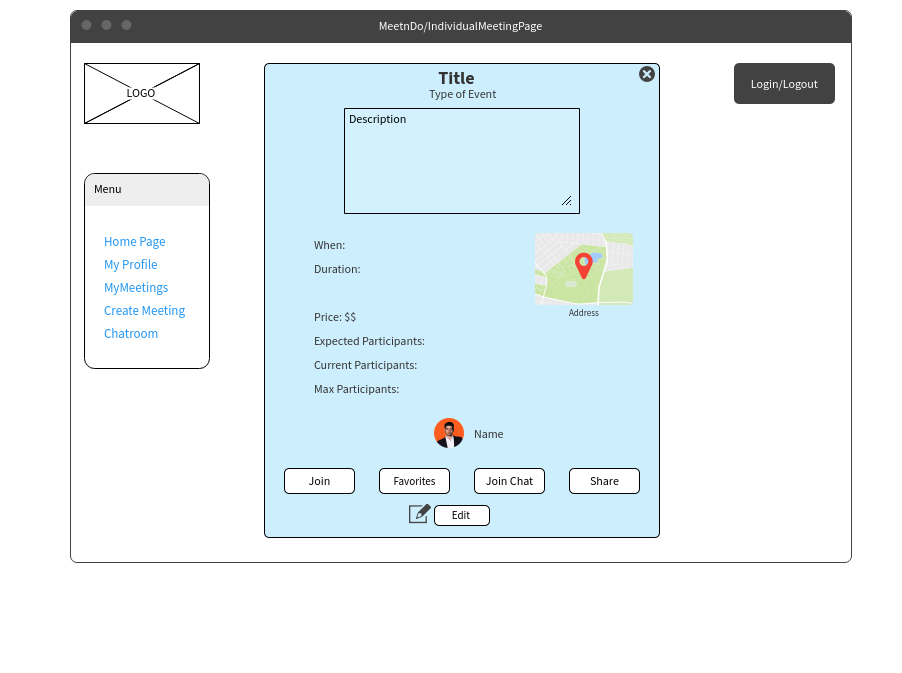
\includegraphics[scale=0.3]{mockups/IndivMeeting}\quad
  \caption { Individual meeting page}
\end{figure}

\begin{figure}
  \centering
  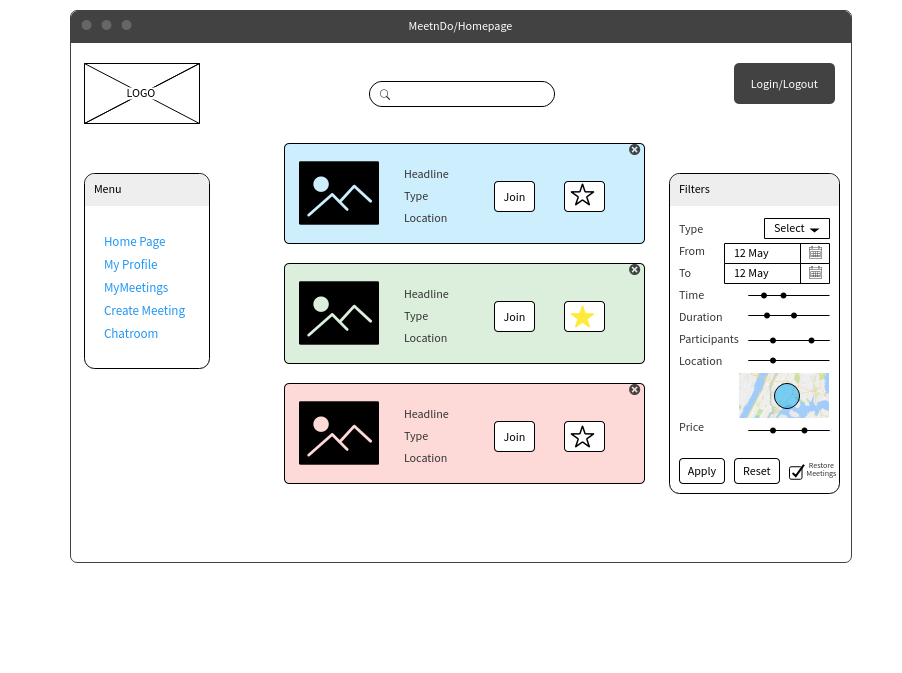
\includegraphics[scale=0.3]{meetndo/pics/mockups/Homepage.png}\quad
  \caption { Homepage}
\end{figure}

\begin{figure}
  \centering
  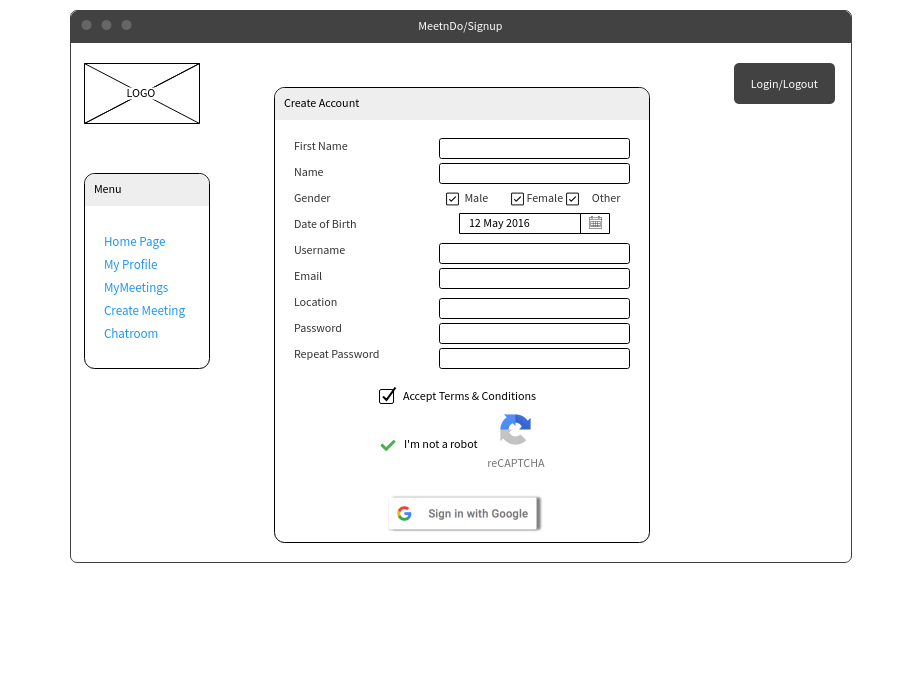
\includegraphics[scale=0.3]{meetndo/pics/mockups/Signup.png}\quad
  \caption { Signup page}
\end{figure}

\begin{figure}
  \centering
  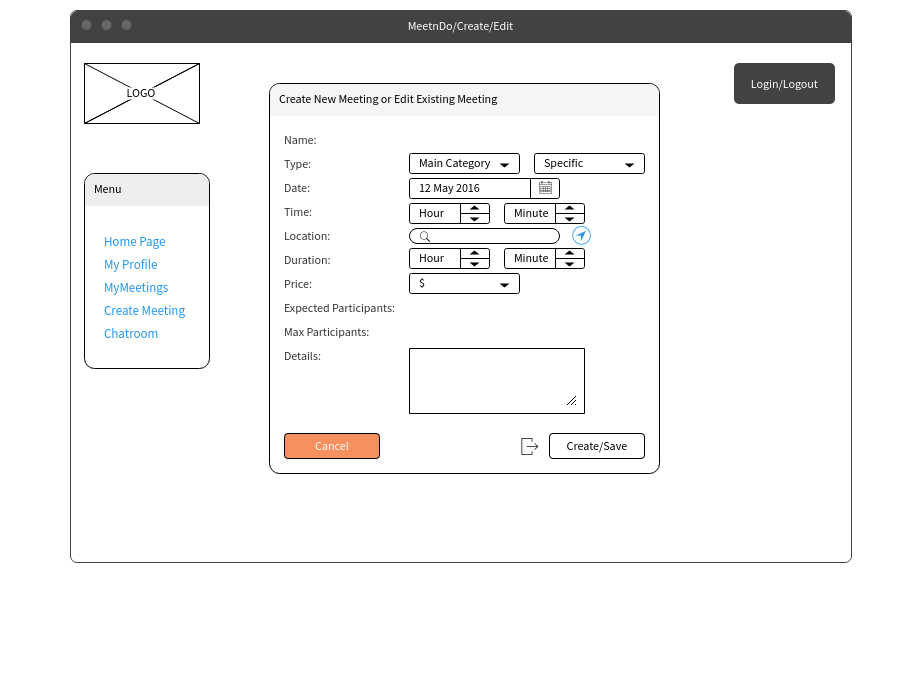
\includegraphics[scale=0.3]{meetndo/pics/mockups/Create_edit.png}\quad
  \caption { Create and Edit Meetings}
\end{figure}

\begin{figure}
  \centering
  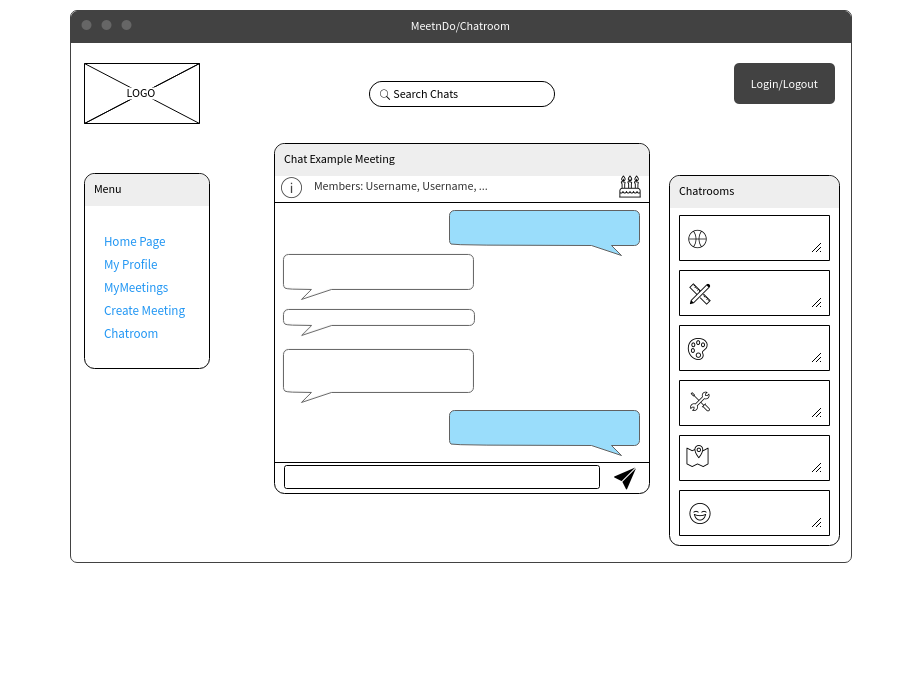
\includegraphics[scale=0.3]{meetndo/pics/mockups/Chatroom.png}\quad
  \caption { Chatroom page}
\end{figure}

\begin{figure}
  \centering
  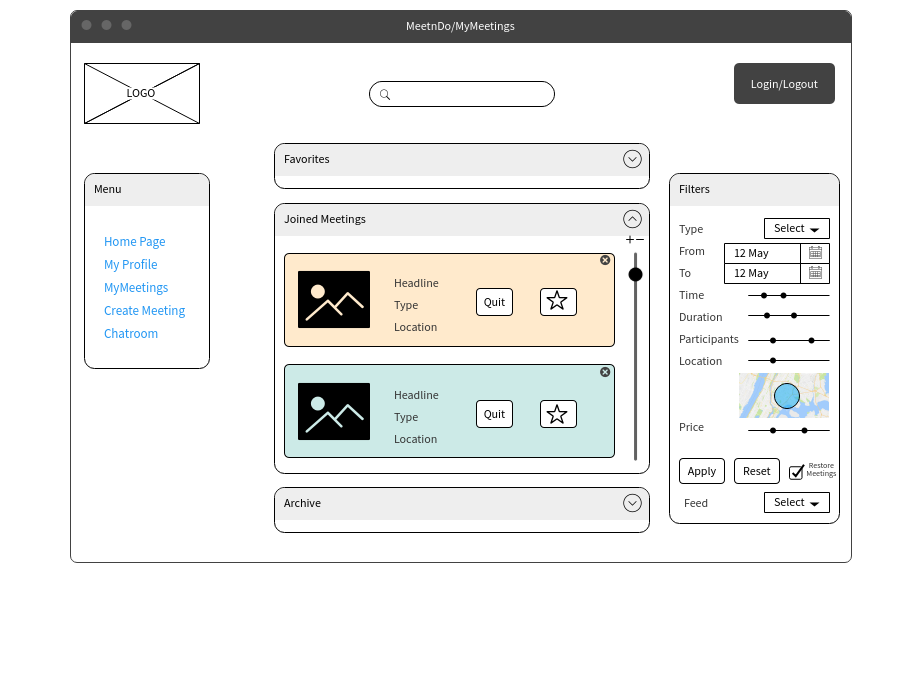
\includegraphics[scale=0.3]{meetndo/pics/mockups/Mymeetings.png}\quad
  \caption { MyMeetings User Meeting page}
\end{figure}

\begin{figure}
  \centering
  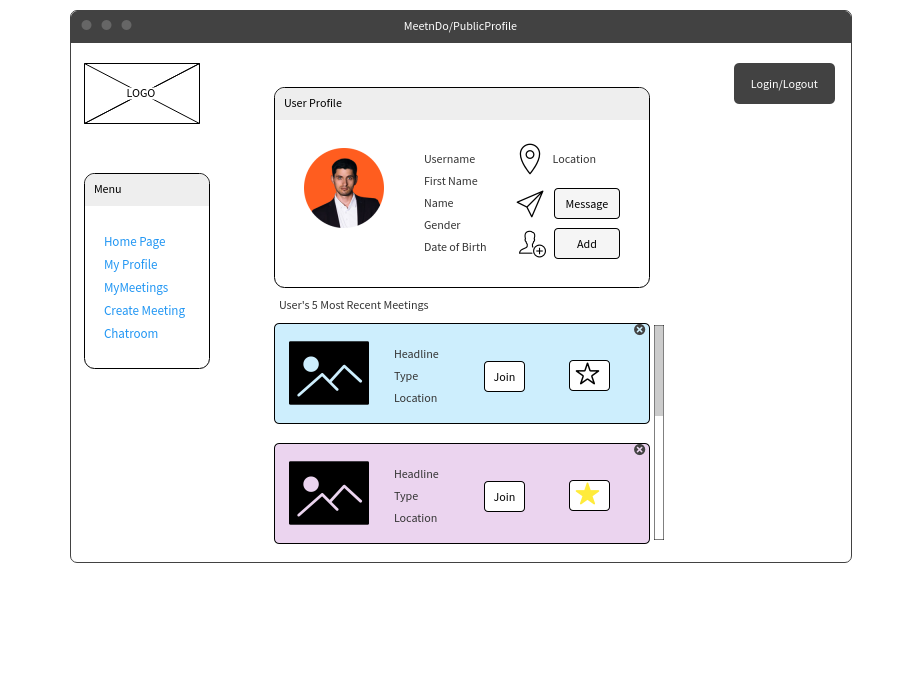
\includegraphics[scale=0.3]{meetndo/pics/mockups/PublicProfile.png}\quad
  \caption { Public Profile page}
\end{figure}

\begin{figure}
  \centering
  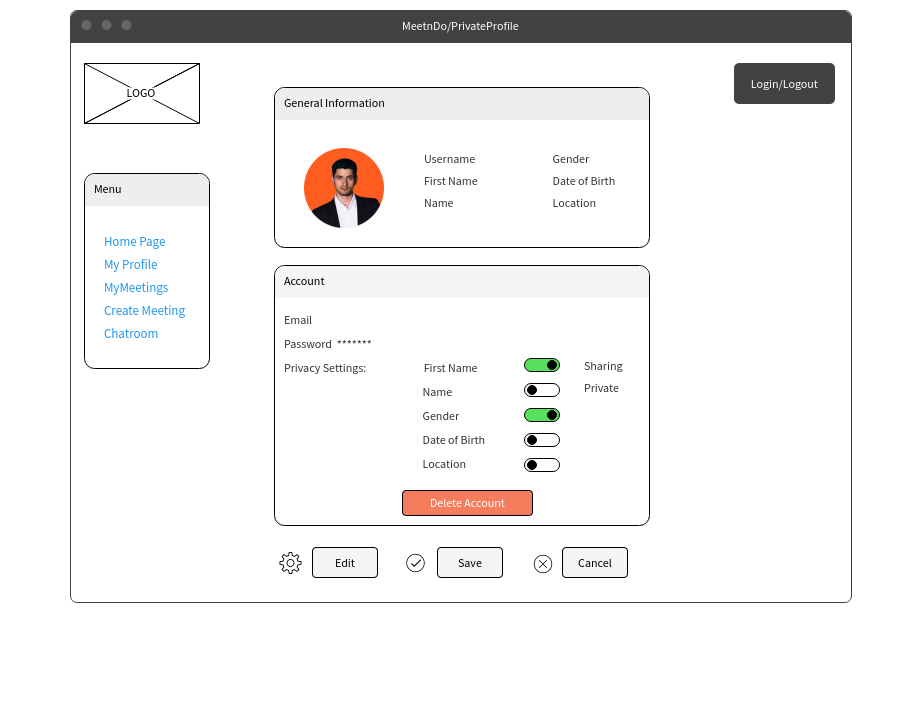
\includegraphics[scale=0.3]{meetndo/pics/mockups/PrivateProfile.png}\quad
  \caption { Private Profile page}
\end{figure}

\clearpage

\subsection{ER Diagram, Class Diagram and Use Case Diagram}

\subsubsection{ER Diagram}

Meetings table: 
This table should contain all the necessary information of a meeting (1 entry per meeting), it’s type is an Integer value referring to the types table which contains all the different types of meetings. The current participant number can be computed when requested so it doesn’t need to be stored in this table. The location entry is a string referring to the Google Places API ID of the selected place.

Users table:
The users table should contain all the information about users (1 entry per user). The location entry is a string referring to the Google Places API ID of the selected city. The privacy entry is a binary value describing the user’s privacy settings: some of the user personal information can be set as either Public or Private like the name/first name, gender, date of birth, email, location, and previous meetings so 6 information in total. For example if every information is set as public the binary should be set to 0x000000 and if 2 of the 6 information are set to private the privacy binary should be set to 0x001010 for example.

Messages table:
This table should contain all relevant information of sent messages within chat rooms (1 entry/message sent). The sender and chatroom values are Integer referring to the sender’s user ID and to the chatroom’s ID.

Chatrooms table:
This table contains all chat rooms (1 entry/chatroom). 
The only information that it stores is if the chatroom is a group chat or a private chat (between 2 users only).

Relations table:
The relations table contains all different relations between a user and a meeting. There are 4 different types of relation: 0 -> Organizer, 1 -> Participant, 2 -> Favorites (The meeting is in the user’s favorites meetings), 3 -> Pending (User made a request to join the meeting but has no confirmation yet). This table is static meaning that it will not change unless new types of relations are added in future versions of the website.

Types table:
The types table contains the name of all different meeting types. The main categories: Food, Sport, Education, Entertainment, Art, Outdoors, Others having a parent value equal to 0 and the sub-categories such as Dinner, Lunch, Swimming, Football, Others that will have a parent value set to the related main category’s ID. This table is also static and doesn’t change unless some new categories are added, or the table is replaced in a future version of the website.

Join tables:
'users\_meetings' and 'users\_chatrooms' tables describe all links between users and meetings and the ones between users and chatrooms. The users\_meetings table additional information for each relation between a user and a table is the type of relation between both entities. The additional information in the users\_chatrooms table is a Boolean stating if the user is the administrator of the chat or not (the organizer of a meeting chat is the administrator, he can decide whether accepting or denying a request to join the meeting from a user from the chatroom).

\subsubsection{Use Case Diagram}

The Use Case Diagram specifies three different roles for the beginning, the need for more positions and further use cases may arise later. Those cases include site users, customer service staff and an administrative position which is necessary for the site to function properly. The customer service role will require hiring staff. Users are able to use all the features of the website such as interacting with meeting participating in chats or create their personal profile. Also, users have to ability to contact customer service staff to resolve any problems or complaints. The role of customer service staff involves answering customer inquiries and managing content as well as users. If necessary, staff will remove or hide inappropriate content. Both customer service and users have the ability to manage account settings. Customer service also serves as a mediator between the users and administrator. The administrator should not be involved in dealing with users and content, as this role consists of managing technical aspects of website and database as well as developing and implementing new features. 
All use cases involve log in/log out from the system with authentification.

\clearpage
\begin{figure}[h!]
  \centering
  \fbox{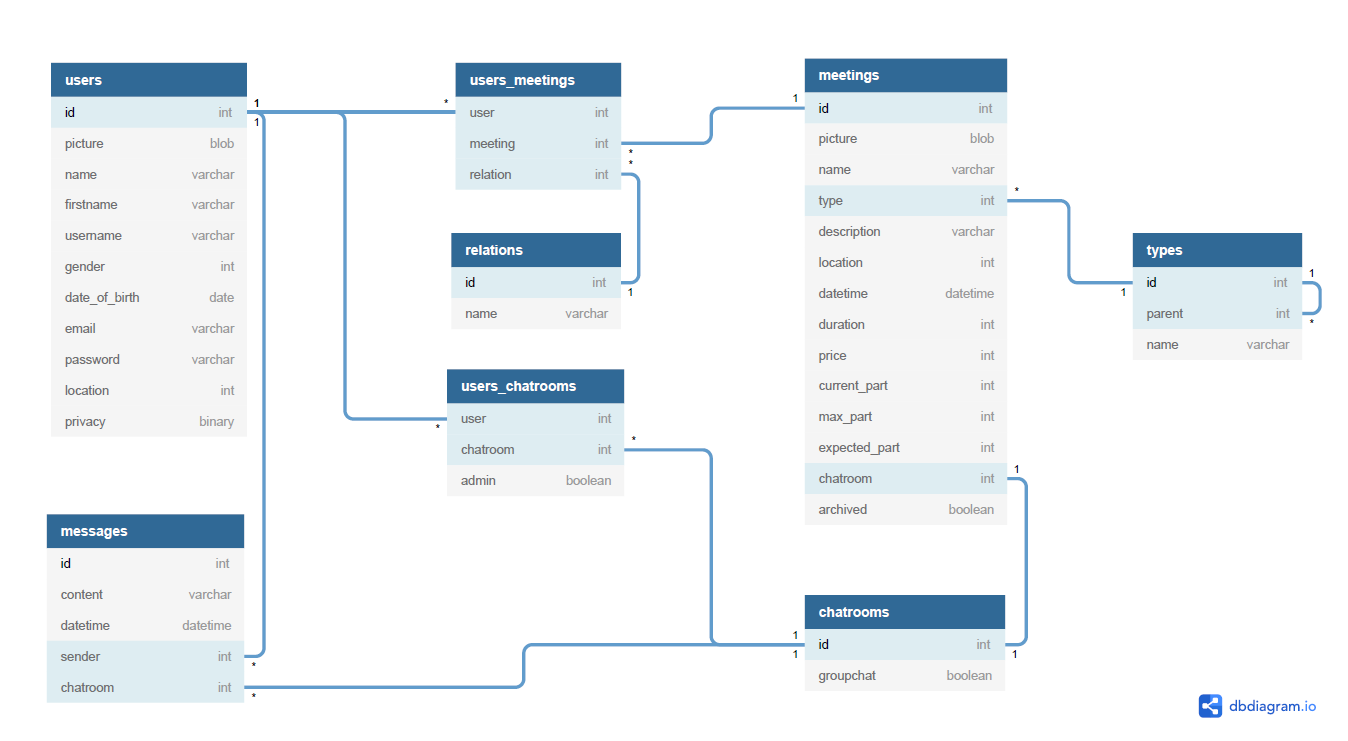
\includegraphics[scale=0.75]{meetndo/pics/diagrams/erdiagram.png}}
  \caption { Meetndo ER Diagram}
\end{figure}


\begin{figure}[h!]
  \centering
  \fbox{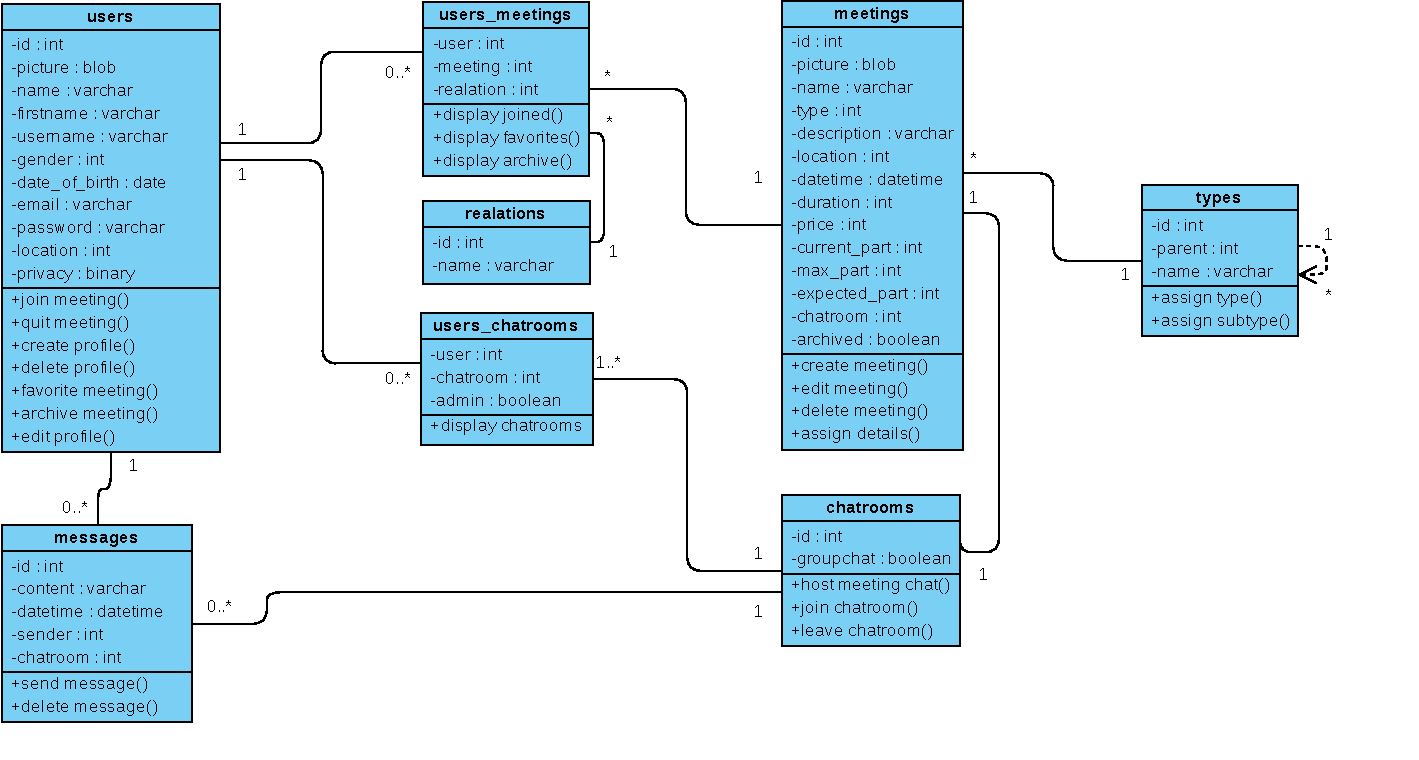
\includegraphics[scale=0.75]{meetndo/pics/diagrams/meetndo_class.pdf}}
  \caption { Meetndo Class Diagram}
\end{figure}

\clearpage
\begin{figure}[h!]
  \centering
  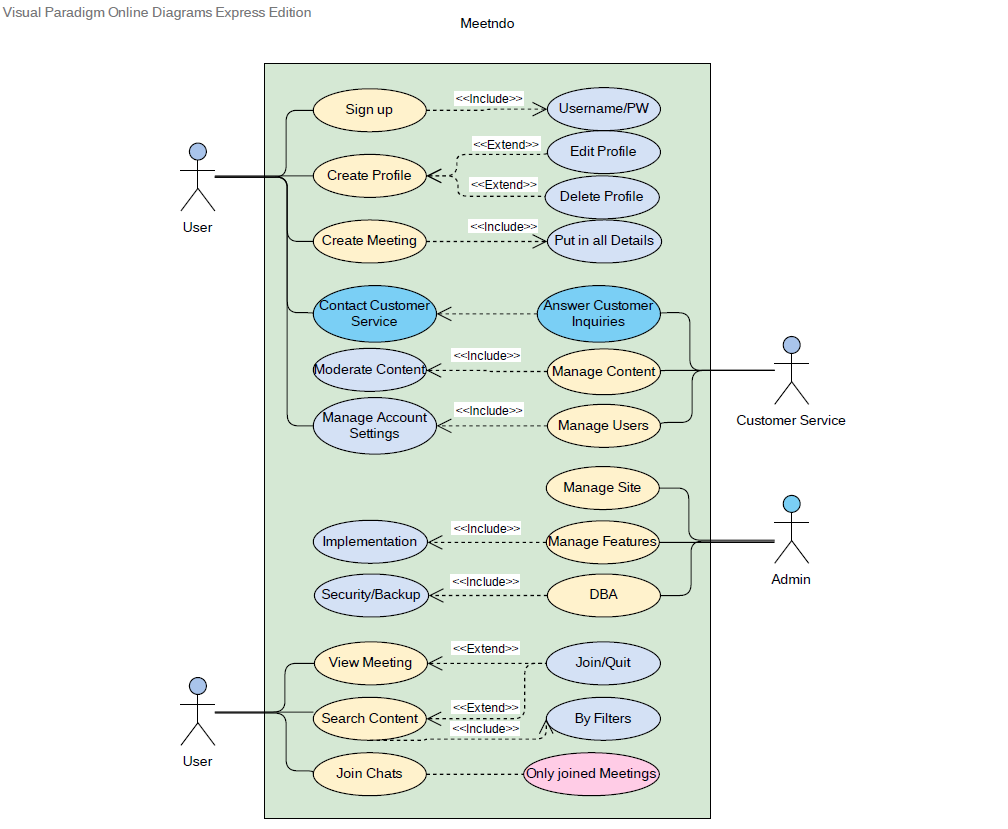
\includegraphics[scale=0.9]{meetndo/pics/diagrams/use_cases.png}
  \caption { Meetndo Use Case Diagram}
\end{figure}


\subsection{Entity Relationship diagram}

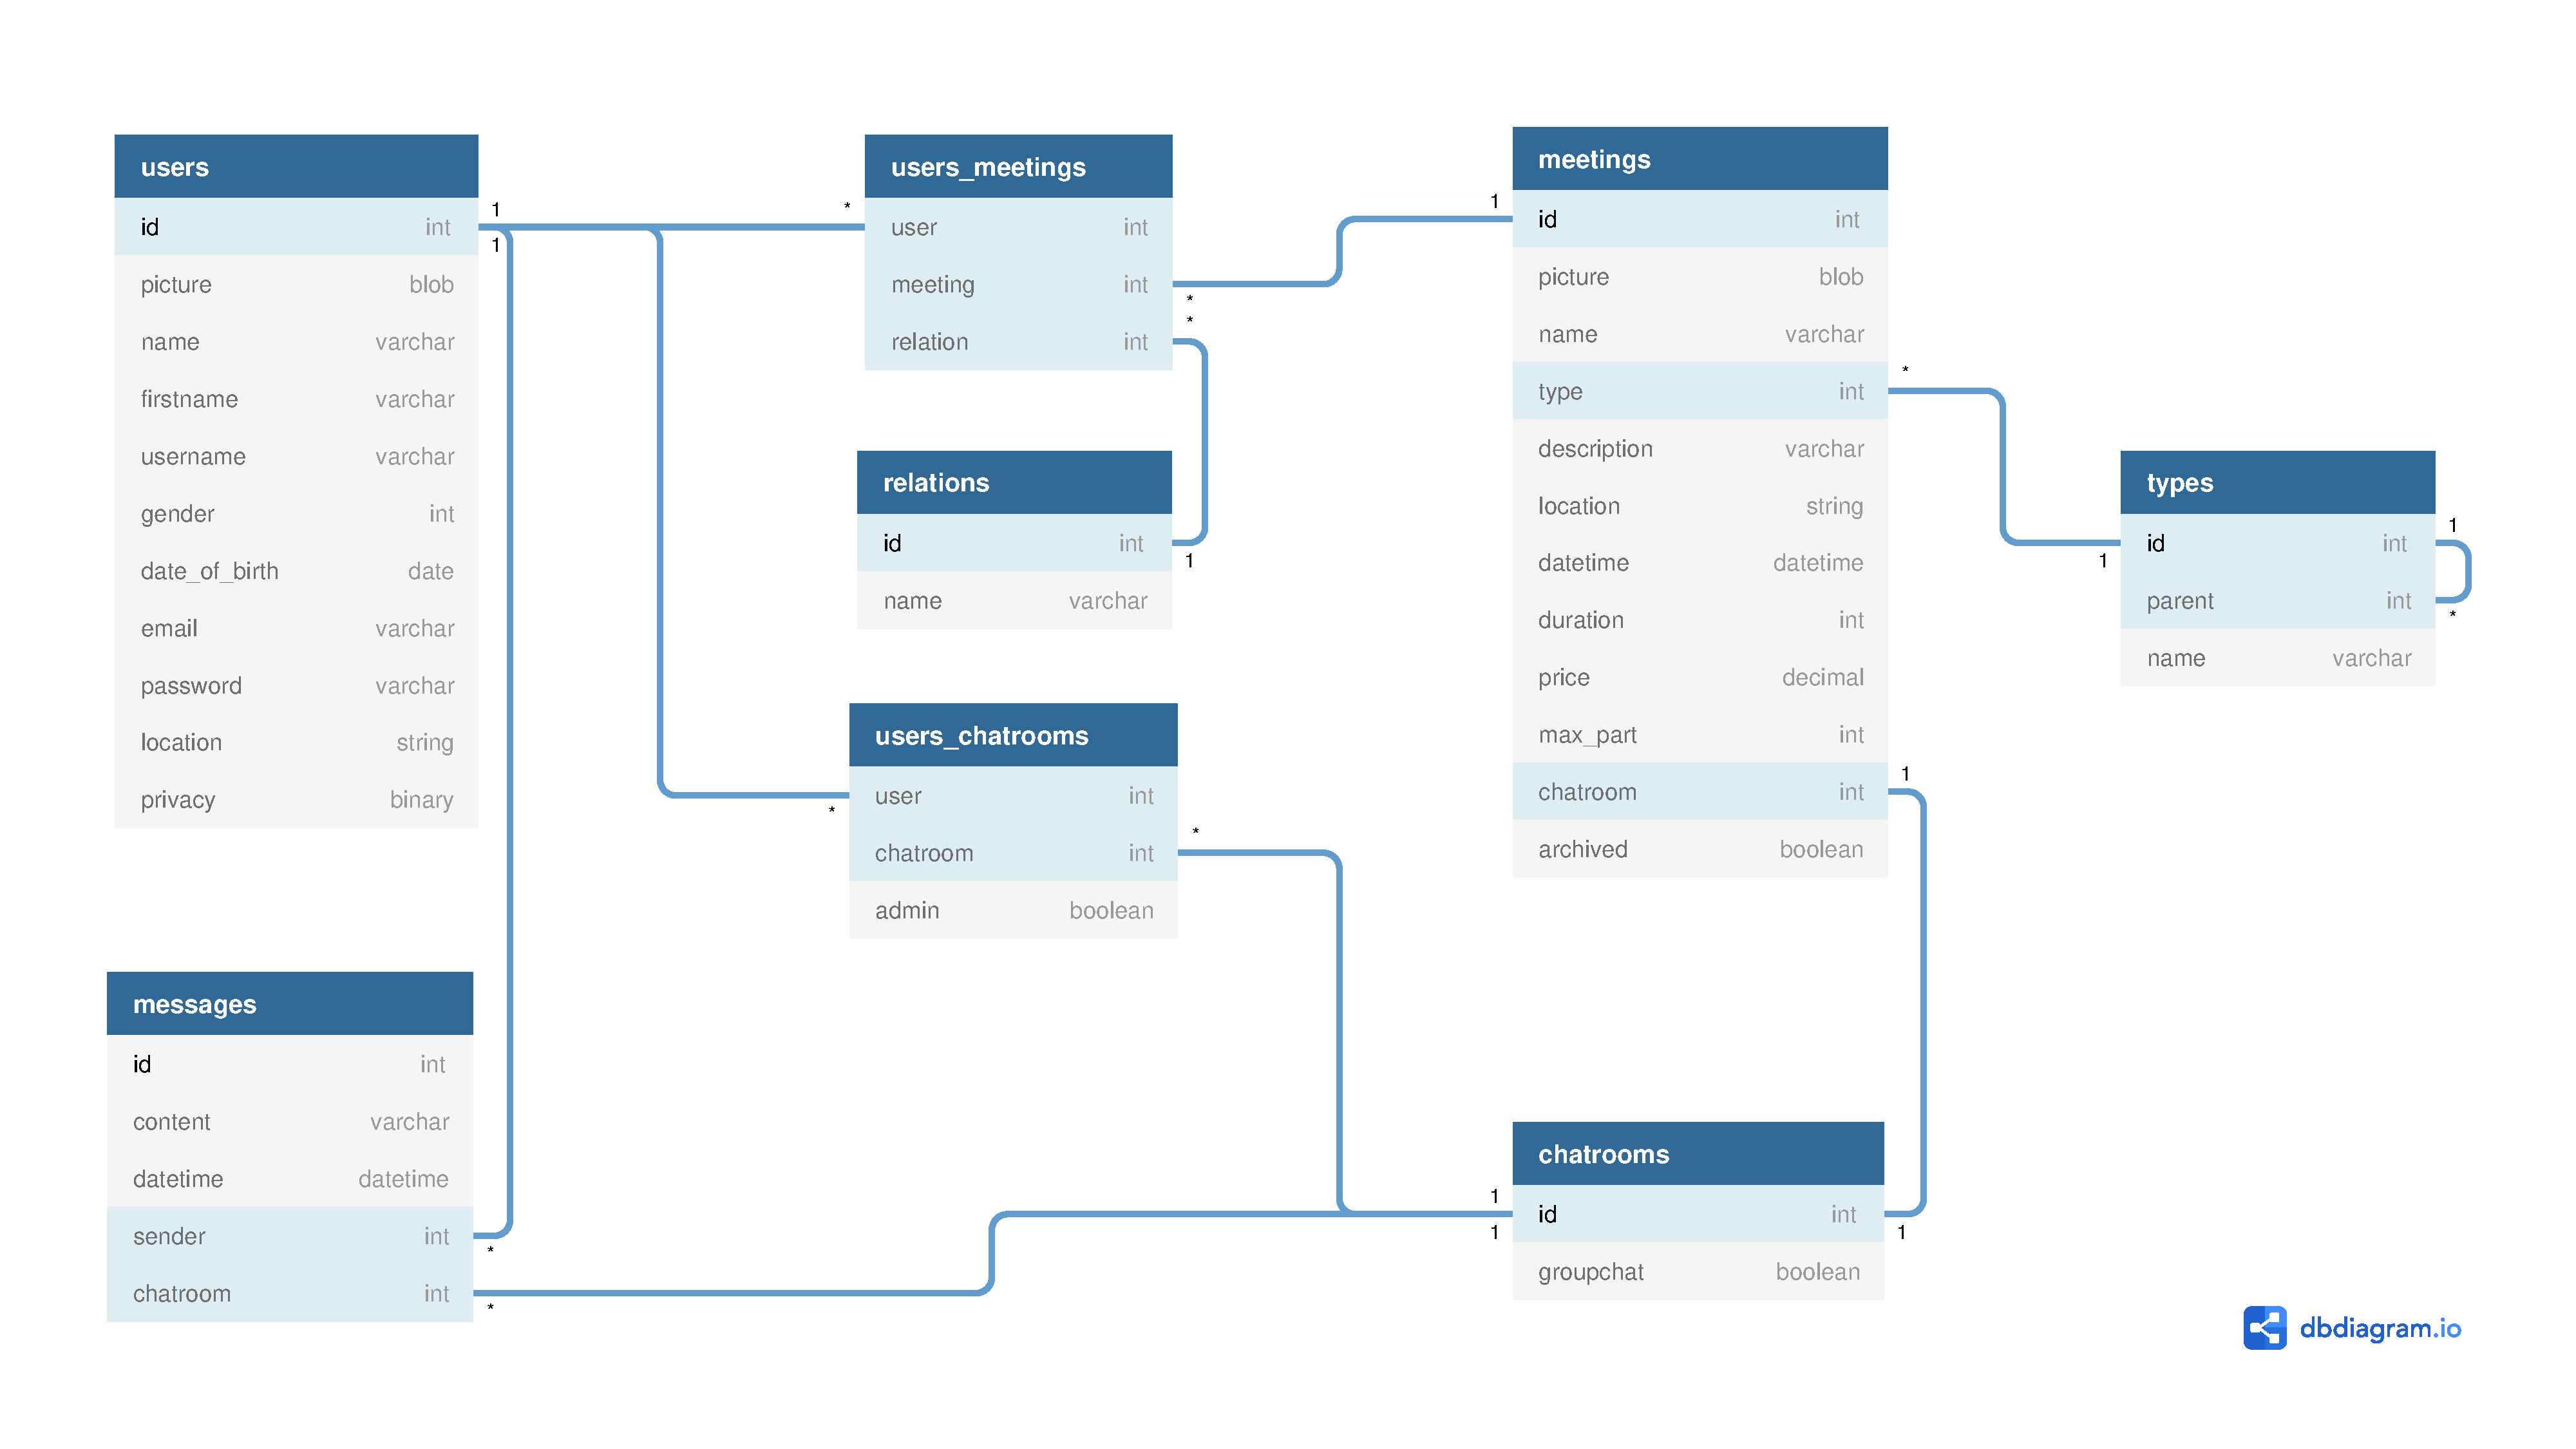
\includepdf[scale=0.5]{ERdiagram/ERdiagram.pdf}

Meetings table: 
This table should contain all the necessary information of a meeting (1 entry per meeting), it’s type is an Integer value referring to the types table which contains all the different types of meetings. The current participant number can be computed when requested so it doesn’t need to be stored in this table. The location entry is a string referring to the Google Places API ID of the selected place.

Users table:
The users table should contain all the information about users (1 entry per user). The location entry is a string referring to the Google Places API ID of the selected city. The privacy entry is a binary value describing the user’s privacy settings: some of the user personal information can be set as either Public or Private like the name/first name, gender, date of birth, email, location, and previous meetings so 6 information in total. For example if every information is set as public the binary should be set to 0x000000 and if 2 of the 6 information are set to private the privacy binary should be set to 0x001010 for example.

Messages table:
This table should contain all relevant information of sent messages within chat rooms (1 entry/message sent). The sender and chatroom values are Integer referring to the sender’s user ID and to the chatroom’s ID.

Chatrooms table:
This table contains all chat rooms (1 entry/chatroom). The only information that it stores is if the chatroom is a group chat or a private chat (between 2 users only).

Relations table:
The relations table contains all different relations between a user and a meeting. There are 4 different types of relation: 0 -> Organizer, 1 -> Participant, 2 -> Favorites (The meeting is in the user’s favorites meetings), 3 -> Pending (User made a request to join the meeting but has no confirmation yet). This table is static meaning that it will not change unless new types of relations are added in future versions of the website.

Types table:
The types table contains the name of all different meeting types. The main categories: Food, Sport, Education, Entertainment, Art, Outdoors, Others having a parent value equal to 0 and the sub-categories such as Dinner, Lunch, Swimming, Football, Others that will have a parent value set to the related main category’s ID. This table is also static and doesn’t change unless some new categories are added, or the table is replaced in a future version of the website.

Join tables:
'users\_meetings' and 'users\_chatrooms' tables describe all links between users and meetings and the ones between users and chatrooms. The users\_meetings table additional information for each relation between a user and a table is the type of relation between both entities. The additional information in the users\_chatrooms table is a Boolean stating if the user is the administrator of the chat or not (the organizer of a meeting chat is the administrator, he can decide whether accepting or denying a request to join the meeting from a user from the chatroom).

\end{document}